\documentclass[11pt,a4paper,twocolumn]{article}

% === Core Packages ===
\usepackage[margin=2cm]{geometry}
\usepackage[utf8]{inputenc}
\usepackage[T1]{fontenc}
\usepackage{times}
\usepackage{amsmath,amssymb}
\usepackage{graphicx}
\usepackage{booktabs}
\usepackage{float}
\usepackage{enumitem}
\usepackage{tikz}
\usepackage{pgfplots}
\pgfplotsset{compat=1.18}
\usetikzlibrary{arrows.meta,shapes.geometric,positioning,calc,decorations.markings,fit,backgrounds}

% === Citation (IEEE style) ===
\usepackage[numbers,sort&compress]{natbib}
\bibliographystyle{IEEEtranN}

% === Hyperref ===
\usepackage[hidelinks]{hyperref}
\usepackage{xurl}

% === Settings ===
\setlength{\parindent}{1em}
\setlength{\parskip}{0.3em}

% === Title ===
\title{\textbf{Rangkaian Reputasi Ternyahpusat:\\Suatu Kerangka Kerja untuk Penyusunan Masyarakat Semula Jadi}}
\author{Pavel Kudrna\\Prague, Czechia\\Draf v1 --- Mac 2026}
\date{}

\begin{document}
\maketitle

% ============================================================
% ABSTRACT
% ============================================================
\begin{abstract}
Rasa keadilan---keyakinan bahawa kesalahan diperbetulkan dan jasa diberi ganjaran---merupakan daya perpaduan masyarakat yang paling kuat. Apabila institusi tadbir urus terpusat tidak dapat menyampaikan rasa ini kerana kos menguatkuasakan sesuatu hak melebihi nilai hak itu sendiri, perpaduan sosial menjadi terhakis. Struktur institusi semasa gagal menyelesaikan satu kelas pertikaian yang ketara dengan cara yang secara sistematik sama seperti perancangan pusat gagal memperuntukkan sumber: melalui ketaksimetrian maklumat, gelung maklum balas yang hilang, dan pemisahan pembuat keputusan daripada akibat keputusan mereka. Kertas ini membentangkan Rangkaian Sosial Reputasi (RSN): suatu lapisan komunikasi ternyahpusat, tidak boleh dirasuah, dan tahan penapisan yang dibina di atas Pengecam Ternyahpusat (DID) yang membolehkan peserta samaran menerbit, mengesah, dan mengguna maklumat reputasi tentang tingkah laku dunia nyata. Mekanisme teras bertumpu pada tiga prinsip reka bentuk: (1)~struktur kos tidak simetri di mana membaca data reputasi adalah murah tetapi menulis memerlukan usaha yang boleh disahkan; (2)~protokol pemilihan pengesah tidak berketentuan berdasarkan pencincangan konsisten yang meletakkan harga pada dakwaan radikal melalui kos lelaran yang meningkat; dan (3)~model autoriti reputasi dipacu pasaran di mana pengesah persendirian mempertaruhkan reputasi terkumpul mereka atas ketepatan dakwaan yang mereka sokong. Seni bina yang terhasil menghasilkan meritokrasi muncul tanpa penyelarasan pusat dan membolehkan laluan peralihan beransur-ansur dan boleh diterbalikkan daripada sistem yang ditadbir oleh negara sedia ada.
\end{abstract}

% ============================================================
% 1. INTRODUCTION
% ============================================================
\section{Pengenalan}

\subsection{Masalah Kepercayaan Terpusat}

Tadbir urus moden bertumpu pada satu andaian asas: bahawa institusi terpusat boleh menjadi pengantara kepercayaan antara orang asing pada skala besar. Mahkamah menghakimi pertikaian. Daftar mengesahkan pemilikan. Badan kawal selia menguatkuasakan piawaian. Institusi-institusi ini direka pada era ketika maklumat adalah terhad, komunikasi adalah lambat, dan pewakilan kuasa kepada badan pusat merupakan satu-satunya mekanisme penyelarasan yang boleh dilaksanakan. Walau bagaimanapun, tadbir urus terpusat gagal atas sebab struktur yang sama seperti perancangan pusat: ketaksimetrian maklumat, gelung maklum balas yang hilang, dan pemisahan pembuat keputusan daripada akibat keputusan mereka.

Andaian ini gagal, sebagai contoh, apabila kos pengantaraan institusi melebihi nilai pertikaian. Pertimbangkan seorang penyewa yang mendapati bahawa apartmen sewaan mereka tiada sijil keselamatan elektrik yang dikehendaki oleh undang-undang---suatu keadaan yang menimbulkan bahaya segera kepada nyawa. Hak undang-undang penyewa untuk menarik diri daripada kontrak adalah jelas. Namun kos menguatkuasakan hak itu melalui sistem mahkamah melebihi nilai kewangan deposit dan ganti rugi yang terhutang, walaupun termasuk potensi pampasan berkanun~\cite{czcourtfees}. Tindak balas yang rasional ialah menanggung kerugian dan keluar.

Ini bukan kes tepi yang patologi. Ia merupakan pengalaman lalai bagi satu kelas pertikaian yang ketara di mana kemudaratan adalah nyata tetapi pertaruhan kewangan jatuh di bawah ambang di mana penguatkuasaan institusi menjadi rasional dari segi ekonomi. Hasilnya ialah suatu sistem yang secara struktur memihak kepada pelaku jahat: mereka yang memudaratkan orang lain dalam jumlah di bawah ambang ini boleh bertindak tanpa hukuman, kerana kos menuntut keadilan jatuh ke atas pihak yang dimudaratkan.

Contoh di atas diambil daripada persekitaran undang-undang penulis---sistem undang-undang sivil Czech. Dalam tradisi undang-undang lain---undang-undang lazim berasaskan duluan, undang-undang adat, sistem campuran---keadilan gagal dengan cara yang berbeza dan pada darjah yang berbeza, bergantung pada kekhususan budaya dan prosedur bidang kuasa tersebut. Pembaca kemungkinan akan mengenali contoh setara daripada konteks mereka sendiri. Apa yang universal dari segi struktur ialah coraknya: pertikaian yang nilainya jatuh di bawah ambang penguatkuasaan yang rasional dari segi ekonomi berakhir dengan kerugian ditanggung oleh pihak yang dimudaratkan. RSN tidak menjanjikan keadilan yang sempurna---ia sekadar mengurangkan kelebihan struktur yang dinikmati oleh pelaku jahat apabila penguatkuasaan institusi tidak ekonomik.

\subsection{Mengapa Penyelesaian Sedia Ada Tidak Mencukupi}

\textbf{Kerangka kerja Identiti Ternyahpusat (DID)}~\cite{did2022} menyediakan mekanisme kriptografi untuk pengurusan identiti berdaulat sendiri tetapi tertumpu terutamanya pada pengesahan identiti tanpa menangani persoalan lebih luas tentang reputasi tingkah laku.

\textbf{Token Terikat Jiwa (SBT)}~\cite{weyl2022} menangkap wawasan bahawa reputasi tidak boleh dipindah milik tetapi bergantung pada infrastruktur blockchain dengan kekangan keterukuran dan tidak menangani insentif ekonomi yang mengawal kemasukan maklumat. Konsep berkaitan seperti token merit (contohnya, Liberland) berkongsi falsafah yang serupa tetapi kekal terikat pada kerangka bidang kuasa tertentu.

\textbf{Organisasi Autonomi Ternyahpusat (DAO)}~\cite{buterin2014} melaksanakan tadbir urus melalui kontrak pintar tetapi mengulangi dinamik plutokratik di mana pengaruh adalah berkadaran dengan modal. Pengundian kuadratik~\cite{buterin2019} sebahagiannya mengurangkan hal ini tetapi mengehadkan penerimaan praktikal. DAO juga menghadapi \emph{masalah orakel} yang asas: kontrak pintar tidak dapat mengesahkan keadaan dunia nyata dengan boleh dipercayai tanpa sumber luaran yang dipercayai, dan masalah ini tiada penyelesaian umum dalam seni bina blockchain.

Tiada sistem sedia ada yang menggabungkan penyahpusatan, ketahanan penapisan, kesamaran, kos kemasukan yang boleh disahkan, dan konsensus yang muncul.

\subsection{Sumbangan}

Kertas ini memberikan sumbangan berikut:
\begin{enumerate}[nosep]
\item Takrifan \textbf{Rangkaian Sosial Reputasi (RSN)}, suatu protokol ternyahpusat yang memanjangkan kerangka kerja DID untuk menyokong pertukaran reputasi dua hala.
\item Suatu \textbf{protokol pemilihan pengesah tidak berketentuan} berdasarkan pencincangan konsisten~\cite{karger1997}.
\item \textbf{Prinsip Radikalisme Mahal}, meletakkan harga pada dakwaan mengikut jarak mereka daripada konsensus rangkaian melalui tiga saluran kos yang berganda.
\item Suatu \textbf{model Autoriti Bereputasi} dengan insentif tidak simetri di mana sokongan palsu memakan kos jauh lebih besar secara malapetaka berbanding yuran yang sah.
\item Suatu \textbf{laluan peralihan beransur-ansur} melalui infrastruktur fiskal selari.
\end{enumerate}

% ============================================================
% 2. DESIGN PRINCIPLES
% ============================================================
\section{Prinsip Reka Bentuk}

Seni bina RSN dikekang oleh lima prinsip reka bentuk yang tidak boleh dirunding.

\textbf{Kesinambungan dan Evolusi.} Sistem ini wujud bersama institusi sedia ada semasa tempoh peralihan yang panjangnya tidak tertentu. Peralihan mesti boleh diterbalikkan pada setiap peringkat.

\textbf{Kerelaan dan Tanggungjawab.} Penyertaan adalah sukarela, tetapi kerelaan digandingkan dengan tanggungjawab: seorang peserta yang mengambil alih kawalan sesuatu fungsi institusi serentak mengambil alih kewajipan yang menyertainya.

\textbf{Kepelbagaian dan Neutraliti Budaya.} Konsensus muncul daripada interaksi dua hala, bukan daripada peraturan yang ditetapkan lebih awal oleh pereka sistem.

\textbf{Daya Tahan dan Ketahanan Penapisan.} Kos menapis rangkaian mesti melebihi kos membiarkannya. Hanya totalitarianisme penuh---dengan kos politik dan ekonomi yang membinasakan---boleh menyekat sistem ini.

\textbf{Konsensus dan Penguatkuasaan.} Sistem ini menggabungkan kecenderungan manusia terhadap kepicikan, dendam, dan kepuasan pembalasan sebagai ciri penanggung beban. Salah laku tidak dilarang; ia diberi harga.

% ============================================================
% 3. SYSTEM OVERVIEW
% ============================================================
\section{Gambaran Keseluruhan Sistem}

\subsection{Rangkaian Sosial Reputasi}

RSN ialah suatu lapisan komunikasi ternyahpusat, rakan ke rakan di mana peserta bertukar maklumat yang boleh disahkan tentang tingkah laku dunia nyata. Sifat penakrifnya ialah: infrastruktur ternyahpusat dan tidak boleh ditapis; penyertaan samaran melalui DID; struktur kos tidak simetri (membaca adalah murah, menulis adalah mahal); kebolehsahan kriptografi; dan \textbf{sokongan piawaian}---format boleh dibaca mesin untuk maklumat yang disebarkan melalui rangkaian, untuk perkhidmatan yang ditawarkan oleh autoriti (gubahan dakwaan, sokongan, perkhidmatan saksi), dan untuk format dasar termasuk peraturan untuk menilai reputasi pihak lawan dan menaksir risiko ketidakpadanan dasar (antara tingkah laku yang diisytiharkan dan sebenar).

\subsection{Komponen Seni Bina}

RSN terdiri daripada empat komponen utama (Raj.~\ref{fig:architecture}):
\begin{enumerate}[nosep]
\item \textbf{Lapisan DID.} Identiti peserta dengan peraturan yang diisytiharkan, metadata reputasi, dan penghalaan rangkaian.
\item \textbf{Protokol Dakwaan.} Format berstruktur untuk menerbitkan pernyataan tentang peristiwa dunia nyata.
\item \textbf{Rangkaian Pengesahan.} Protokol ternyahpusat untuk menetapkan pengesah menggunakan pencincangan konsisten.
\item \textbf{Lapisan Pengagregatan Reputasi.} Perkhidmatan yang menghasilkan ringkasan reputasi yang boleh dibaca manusia.
\end{enumerate}

\begin{figure}[ht]
\centering
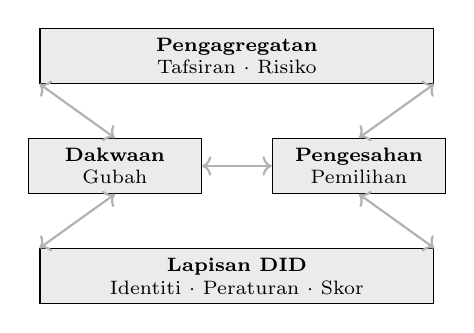
\begin{tikzpicture}[
    layer/.style={draw, minimum height=0.7cm, align=center, font=\scriptsize, fill=black!8},
    arr/.style={<->, thick, gray!60}
]
\node[layer, minimum width=5cm] (agg) at (0,2.8) {\textbf{Pengagregatan}\\Tafsiran\ $\cdot$ Risiko};
\node[layer, minimum width=2.2cm] (claim) at (-1.55,1.4) {\textbf{Dakwaan}\\Gubah};
\node[layer, minimum width=2.2cm] (verif) at (1.55,1.4) {\textbf{Pengesahan}\\Pemilihan};
\node[layer, minimum width=5cm] (did) at (0,0) {\textbf{Lapisan DID}\\Identiti $\cdot$ Peraturan $\cdot$ Skor};

\draw[arr] (agg.south west) -- (claim.north);
\draw[arr] (agg.south east) -- (verif.north);
\draw[arr] (claim.east) -- (verif.west);
\draw[arr] (claim.south) -- (did.north west);
\draw[arr] (verif.south) -- (did.north east);
\end{tikzpicture}
\caption{Seni bina empat lapisan RSN.}
\label{fig:architecture}
\end{figure}

\subsection{Peranan Peserta}

Suatu transaksi pengesahan melibatkan sehingga enam peranan DID yang berbeza (Raj.~\ref{fig:roles}): \textbf{Pengeluar} ($DID_I$, mencipta dan menyerahkan dakwaan), \textbf{Subjek} ($DID_S$, DID yang menjadi subjek dakwaan---mungkin bertindih dengan Pengeluar), \textbf{Autoriti} ($DID_A$, menyokong dakwaan dengan yuran; mungkin juga menawarkan perkhidmatan saksi---\emph{pilihan}), \textbf{Saksi} ($DID_{W_{1..n}}$, pemantau incognito kejujuran pengesah melalui kod cabaran---\emph{pilihan}), \textbf{Pengesah} ($DID_V$, dipilih secara algoritma untuk menerbitkan dakwaan), dan \textbf{RSN} (rangkaian tempat dakwaan yang disahkan diterbitkan). Mana-mana peranan boleh diwakilkan kepada DID lain (Seksyen~7.4). Suatu Autoriti biasanya menggabungkan sokongan dengan perkhidmatan saksi, tetapi kedua-dua fungsi adalah bebas secara logik.

\begin{figure}[ht]
\centering
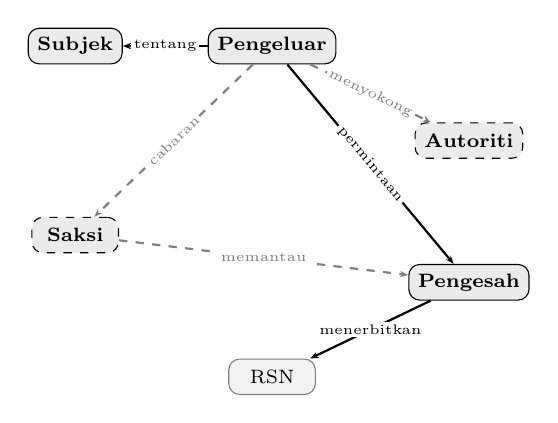
\begin{tikzpicture}[
    role/.style={draw, rounded corners, minimum width=1.1cm, minimum height=0.45cm, align=center, font=\scriptsize, fill=black!8},
    opt/.style={draw, rounded corners, minimum width=1.1cm, minimum height=0.45cm, align=center, font=\scriptsize, fill=black!8, dashed},
    arr/.style={-{Stealth[length=3pt]}, thick},
    oarr/.style={-{Stealth[length=3pt]}, thick, dashed, gray},
    lbl/.style={font=\tiny, fill=white, inner sep=1pt}
]
\node[role] (I) at (0,2.4) {\textbf{Pengeluar}};
\node[role] (S) at (-2.5,2.4) {\textbf{Subjek}};
\node[opt] (A) at (2.5,1.2) {\textbf{Autoriti}};
\node[opt] (W) at (-2.5,0) {\textbf{Saksi}};
\node[role] (V) at (2.5,-0.6) {\textbf{Pengesah}};
\node[role, fill=black!5, draw=gray] (N) at (0,-1.8) {RSN};

\draw[arr] (I) -- node[lbl] {tentang} (S);
\draw[oarr] (I) -- node[lbl,sloped] {menyokong} (A);
\draw[oarr] (I) -- node[lbl,sloped] {cabaran} (W);
\draw[arr] (I) -- node[lbl,sloped] {permintaan} (V);
\draw[oarr] (W) -- node[lbl] {memantau} (V);
\draw[arr] (V) -- node[lbl] {menerbitkan} (N);
\end{tikzpicture}
\caption{Peranan DID dalam suatu transaksi pengesahan. Putus-putus = pilihan (Autoriti, Saksi).}
\label{fig:roles}
\end{figure}

\subsection{Ketidakbolehrasuahan: Empat Daya}

Ketidakbolehrasuahan RSN tidak timbul daripada satu mekanisme tunggal tetapi daripada empat daya serentak. Tiada satu pun mencukupi dengan sendirinya; hanya gabungan mereka menjadikan percubaan rasuah tidak rasional dari segi ekonomi.

\textbf{Sasaran yang tidak dapat diramal.} Pengesah bagi setiap dakwaan dipilih secara tidak berketentuan melalui pencincangan konsisten (Seksyen~5.3). Penyerang tidak dapat menyasarkan pengesah tertentu terlebih dahulu untuk rasuah, kerana identiti pengesah adalah fungsi kandungan dakwaan dan lelaran sebelumnya, bukan pilihan pengeluar.

\textbf{Leveraj reputasi---naik perlahan, turun cepat.} Reputasi hanya boleh diperoleh secara beransur-ansur, melalui tingkah laku konsisten yang berterusan. Namun, ia boleh hilang secara malapetaka dalam satu sokongan penipuan (Seksyen~6.2). Ketaksimetrian ini bermakna bertahun-tahun reputasi terkumpul boleh dimusnahkan oleh satu sokongan yang tidak jujur; strategi optimum kekal untuk menolak dakwaan yang mencurigakan.

\textbf{Janji awam.} Setiap Pemegang DID mengisytiharkan dasar mereka secara terbuka---satu set peraturan boleh dibaca mesin yang mereka komit untuk ikuti. Perbezaan antara pengisytiharan dan tingkah laku sebenar adalah boleh dikesan dan diberi harga sebagai kesalahan reputasi yang lebih teruk daripada pelanggaran asas (Seksyen~7.3). Oleh itu, kemunafikan lebih mahal daripada ketidakjujuran langsung.

\textbf{Ketaksimetrian kos serangan jejaring.} Kos menapis atau menggoyahkan rangkaian bertumbuh secara tidak linear dengan saiz dan ketumpatan rangkaian, sementara kos membiarkannya kekal tetap. Untuk penapisan menjadi berbaloi, seorang pelaku terpusat perlu menggunakannya merentasi seluruh rangkaian---memerlukan langkah yang tidak berkadaran dengan sebarang manfaat yang boleh dibayangkan (Seksyen~10).

% ============================================================
% 4. DECENTRALIZED IDENTITY MODEL
% ============================================================
\section{Model Identiti Ternyahpusat}

\subsection{DID dengan Sifat Khas}

RSN memanjangkan spesifikasi W3C DID Core~\cite{did2022} dengan: \textbf{Peraturan Diisytiharkan} (komitmen tingkah laku boleh dibaca mesin), \textbf{Metadata Reputasi} (skor tingkah laku teragregat), dan \textbf{Penghalaan Rangkaian} (get laluan onion boleh ubah yang berasingan daripada kedudukan gelang yang stabil).

\subsection{Kitaran Hayat Dakwaan}

Suatu Dakwaan melalui enam peringkat (Raj.~\ref{fig:lifecycle}): gubahan, sokongan autoriti pilihan, pemilihan pengesah melalui pencincangan konsisten, keputusan pengesahan (terima atau tolak dengan lelaran), penerbitan, dan kemas kini reputasi untuk semua pihak.

\begin{figure}[ht]
\centering
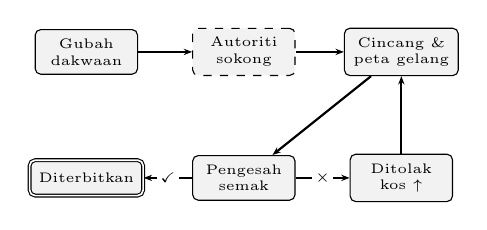
\begin{tikzpicture}[
    stp/.style={draw, rounded corners=2pt, minimum width=1.3cm, minimum height=0.45cm, align=center, font=\tiny, fill=black!5},
    arr/.style={-{Stealth[length=3pt]}, thick},
    lbl/.style={font=\tiny, fill=white, inner sep=1pt}
]
\node[stp] (comp) at (0,0) {Gubah\\dakwaan};
\node[stp, dashed] (auth) at (2.0,0) {Autoriti\\sokong};
\node[stp] (hash) at (4.0,0) {Cincang \&\\peta gelang};
\node[stp] (ver) at (2.0,-1.6) {Pengesah\\semak};
\node[stp, double] (pub) at (0,-1.6) {Diterbitkan};
\node[stp] (rej) at (4.0,-1.6) {Ditolak\\kos $\uparrow$};

\draw[arr] (comp) -- (auth);
\draw[arr] (auth) -- (hash);
\draw[arr] (hash) -- (ver);
\draw[arr] (ver) -- node[lbl] {\checkmark} (pub);
\draw[arr] (ver) -- node[lbl] {$\times$} (rej);
\draw[arr] (rej) -- ++(0,0.8) -| (hash);
\end{tikzpicture}
\caption{Kitaran hayat dakwaan dengan gelung lelaran.}
\label{fig:lifecycle}
\end{figure}

\subsection{Hubungan dengan W3C DID Core}

Model identiti RSN merupakan superset sempurna bagi spesifikasi W3C DID Core~\cite{did2022}. Semua DID RSN adalah DID W3C yang sah. Sambungan khusus RSN dikodkan sebagai sifat dokumen DID yang ditakrifkan dalam spesifikasi kaedah DID yang khusus, serasi dengan infrastruktur sedia ada seperti ION~\cite{buchner2021} dan Ceramic~\cite{ceramic2023}.

% ============================================================
% 5. VERIFICATION AND PROPAGATION
% ============================================================
\section{Pengesahan dan Penyebaran Maklumat}

\subsection{Kos Kemasukan Maklumat}

Prinsip ekonomi teras RSN ialah ketaksimetrian antara membaca dan menulis. Membaca data reputasi menghampiri kos sut sifar bagi peserta yang menjadi sebahagian daripada rangkaian DID dan mempunyai akses yang setara dengan reputasi mereka---pendatang baharu mesti secara beransur-ansur memperoleh akses yang lebih luas (lihat anti-lintah). Menulis---difahami sebagai pewujudan reputasi yang tahan lama ke dalam rangkaian, bukan sebagai satu perbuatan teknikal sekali sahaja---memerlukan pelaburan terkumpul yang boleh disahkan merentasi tiga dimensi: \textbf{masa} (bertahun-tahun kehidupan yang dihabiskan pada tingkah laku konsisten, komitmen yang dipenuhi, dan hubungan yang dibina), \textbf{tenaga} (usaha yang dilaburkan dalam urus niaga jujur, penjagaan perkongsian, dan kebolehpercayaan jangka panjang), dan \textbf{wang} (pelaburan dalam nama sendiri---pembangunan profesional, kualiti kerja seseorang, restitusi atas kemudaratan yang disebabkan). Reputasi tidak boleh dibeli serta-merta---ia adalah hasil pengumpulan sepanjang hayat yang sistem sekadar menjadikannya kelihatan dan boleh dipindahkan merentasi konteks. Kos teknikal sekali sahaja bagi protokol (tandatangan kriptografi, yuran pengesah) adalah tidak ketara berbanding pelaburan asas ini.

\subsection{Graf Sosial dan Kedalaman Kenalan}

RSN pada asasnya ialah suatu rangkaian sosial: setiap DID menambah kenalan (DID lain) yang membenarkan sambungan. Kenalan ini mempunyai kenalan mereka sendiri, dan seterusnya. Carian pengesah algoritma beroperasi dalam kedalaman kenalan berpaut yang boleh dikonfigurasi $h$ (contohnya, $h=3$: kenalan langsung seseorang, kenalan mereka, dan kenalan bagi kenalan). Seni bina ini tidak memerlukan satu blockchain global tunggal---ia secara semula jadi memihak kepada kemunculan komuniti/kelompok dengan pertindihan ke dalam komuniti lain. Setiap peserta DID mesti mempunyai \textbf{dasar} yang diterbitkan---satu set peraturan boleh dibaca mesin yang mengawal bagaimana permintaan masuk dinilai. Pelanggaran dasar direkodkan dalam rangkaian sebagai artifak negatif.

\subsection{Pemilihan Pengesah Algoritma}

Protokol pengesahan menggunakan pencincangan konsisten~\cite{karger1997} (Raj.~\ref{fig:verifier}). Pengesahan ialah perkhidmatan berbayar: pengesah beroperasi dengan yuran, mewujudkan pasaran di mana persaingan memacu penetapan harga, kelajuan, dan kebolehpercayaan.

\textbf{Langkah 1.} Dokumen dakwaan digabungkan dengan hasil cincangan lelaran sebelumnya (atau $\varnothing$ pada lelaran pertama) dan dicincang:
\begin{equation}
\text{pos} = f_h(\text{claim} \| \text{prev\_hash})
\label{eq:hash}
\end{equation}

Algoritma mesti memasukkan \emph{laluan lengkap} bagi semua permintaan dan respons sebelumnya---bukan sekadar cincangan bagi lelaran sebelumnya. Respons penuh setiap pengesah (penerimaan, penolakan, harga yang disebut, sebab) ditambah pada dokumen yang berkembang, boleh disahkan melalui tandatangan kriptografi pada setiap langkah.

\textbf{Langkah 2.} Cincangan dipetakan kepada $N$ kedudukan pada gelang cincangan konsisten, diagihkan sekata (contohnya, untuk $N=4$: $+0^{\circ}, +90^{\circ}, +180^{\circ}, +270^{\circ}$). Daripada setiap kedudukan, carian mengikut pusingan jam memilih DID terdekat sebagai calon pengesah (Raj.~\ref{fig:multipoint}). $N$ ialah parameter berubah yang mungkin bergantung pada peratusan DID yang aktif buat masa ini, waktu dalam sehari, atau kebolehtindakbalasan rangkaian sejarah.

\textbf{Langkah 3.} Pengesah menerima (menerbitkan, mempertaruhkan reputasi) atau menolak (kembali ke Langkah~1 dengan cincangan penolakan). Apabila sesuatu nod tidak bertindak balas walaupun mengisytiharkan status dalam talian, permintaan seterusnya mesti memasukkan semua respons daripada kesemua $N$ calon pengesah sebelumnya.

\textbf{Anti-lintah.} DID sasaran boleh menetapkan yuran atau sekatan akses untuk pertanyaan daripada DID baharu yang mempunyai sedikit reputasi. Mekanisme berperingkat ini (bukan binari) memaksa pendatang baharu membina reputasi melalui aktiviti tulen sebelum bebas menggunakan data orang lain.

\begin{figure}[ht]
\centering
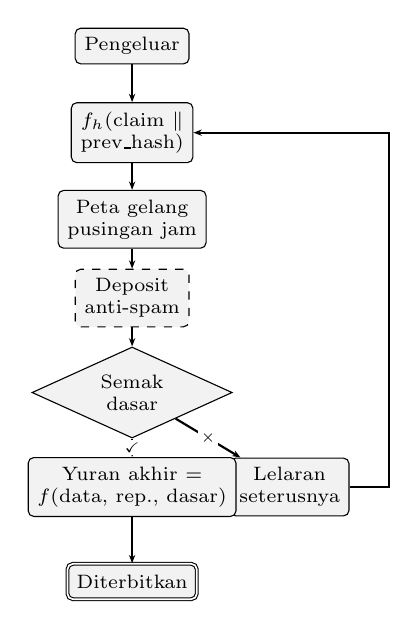
\begin{tikzpicture}[
    box/.style={draw, rounded corners=2pt, minimum width=1.3cm, minimum height=0.45cm, align=center, font=\scriptsize, fill=black!5},
    dec/.style={draw, diamond, aspect=2.2, minimum width=0.9cm, align=center, font=\scriptsize, fill=black!5},
    arr/.style={-{Stealth[length=3pt]}, thick},
    lbl/.style={font=\tiny, fill=white, inner sep=1pt}
]
\node[box] (iss) at (0,0) {Pengeluar};
\node[box] (hash) at (0,-1.1) {$f_h$(claim $\|$\\prev\_hash)};
\node[box] (ring) at (0,-2.2) {Peta gelang\\pusingan jam};
\node[box, dashed] (spam) at (0,-3.2) {Deposit\\anti-spam};
\node[dec] (check) at (0,-4.4) {Semak\\dasar};
\node[box] (rej) at (2,-5.6) {Lelaran\\seterusnya};
\node[box] (fee) at (0,-5.6) {Yuran akhir =\\$f$(data, rep., dasar)};
\node[box, double] (pub) at (0,-6.8) {Diterbitkan};

\draw[arr] (iss) -- (hash);
\draw[arr] (hash) -- (ring);
\draw[arr] (ring) -- (spam);
\draw[arr] (spam) -- (check);
\draw[arr] (check) -- node[lbl] {$\times$} (rej);
\draw[arr] (check) -- node[lbl] {\checkmark} (fee);
\draw[arr] (fee) -- (pub);
\draw[arr] (rej.east) -- ++(0.5,0) |- (hash.east);
\end{tikzpicture}
\caption{Protokol pemilihan pengesah. Deposit anti-spam adalah pilihan dan mungkin boleh dikembalikan. Yuran akhir dibayar hanya semasa penerimaan.}
\label{fig:verifier}
\end{figure}

Setiap penolakan menambah respons penuh pengesah (termasuk sebab dan syarat) pada dokumen dakwaan, mengembangkan kandungannya. Daripada dokumen yang dikembangkan, satu cincangan baharu dikira secara tidak berketentuan, memetakan kepada kedudukan gelang yang berbeza dan memilih pengesah yang berbeza. Pendokumenan laluan penuh adalah wajib---pengeluar tidak dapat meramal atau mempengaruhi pengesah seterusnya. Jika seorang pengesah mengabaikan permintaan walaupun mempunyai dasar diisytihar yang serasi, saksi (jika ada) merekodkan hal ini, dan pengeluar boleh melampirkan bukti saksi semasa penerbitan akhir.

\begin{figure}[ht]
\centering
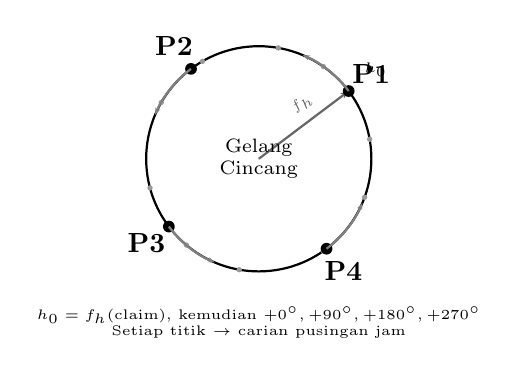
\begin{tikzpicture}[scale=0.65]
% Ring
\draw[thick] (0,0) circle (2.2cm);
% DID nodes on ring
\foreach \a in {10,55,80,120,150,195,230,260,305,340} {
  \fill[black!40] (\a:2.2) circle (1.5pt);
}
% Hash offset arrow pointing to initial position
\draw[-{Stealth[length=3pt]}, thick, black!60] (0,0) -- node[font=\tiny,above,sloped,pos=0.6] {$f_h$} (37:2.2);
\fill[black] (37:2.2) circle (2pt);
\node[font=\tiny,anchor=south west] at (37:2.35) {$h_0$};
% N=4 points offset from h0 by +0, +90, +180, +270
\foreach \offset/\l in {0/P1,90/P2,180/P3,270/P4} {
  \pgfmathsetmacro{\ang}{37+\offset}
  \node[fill=black, circle, inner sep=1.5pt] (p\offset) at (\ang:2.2) {};
  \node[font=\tiny,font=\bfseries] at (\ang:2.75) {\l};
  % clockwise search arc
  \draw[-{Stealth[length=2.5pt]}, thick, gray] (\ang:2.2) arc (\ang:\ang+30:2.2);
}
\node[font=\scriptsize, align=center] at (0,0) {Gelang\\Cincang};
\node[font=\tiny, align=center] at (0,-3.2) {$h_0 = f_h(\text{claim})$, kemudian $+0^{\circ},+90^{\circ},+180^{\circ},+270^{\circ}$\\Setiap titik $\rightarrow$ carian pusingan jam};
\end{tikzpicture}
\caption{Pemilihan berbilang titik ($N{=}4$). Cincangan $h_0$ menetapkan ofset; 4 titik diagihkan sekata daripada $h_0$.}
\label{fig:multipoint}
\end{figure}

\subsection{Protokol Saksi}

Peranan \textbf{Saksi} menyediakan kebertanggungjawaban incognito bagi kejujuran pengesah melalui protokol kod cabaran kriptografi:

\textbf{Langkah W1.} Pemohon menandatangani permintaan pengesahan dan menghantarnya kepada $N_w$ saksi---kenalan daripada rangkaian sosial pemohon, atau penyedia perkhidmatan saksi khusus yang beroperasi dengan yuran.

\textbf{Langkah W2.} Setiap saksi $w_i$ menandatangani keseluruhan permintaan yang telah ditandatangani, menyimpan tandatangan asal $\sigma_i$, dan mengira kod cabaran $c_i = h(\sigma_i)$. Kod cabaran ditambah pada permintaan.

\textbf{Langkah W3.} Permintaan, kini membawa $N_w$ kod cabaran, dihantar kepada pengesah. Pengesah memerhati kod-kod itu tetapi \emph{tidak dapat menentukan} siapa saksi tersebut atau sama ada kod itu sepadan dengan tandatangan sebenar.

\textbf{Langkah W4 (pengesah jujur).} Jika pengesah bertindak balas mengikut dasar diisytihar mereka, kod cabaran kekal legap. Saksi tidak pernah didedahkan. Tiada data tambahan diterbitkan.

\textbf{Langkah W5 (pelanggaran dasar).} Jika pengesah melanggar dasar mereka (mengabaikan permintaan, bertindak balas secara tidak konsisten), pemohon memegang tandatangan asal saksi $\sigma_i$. Ini boleh diterbitkan sebagai data pendamping: sesiapa sahaja boleh mengesahkan $c_i = h(\sigma_i)$, membuktikan saksi hadir. Pemohon boleh menerbitkan secara bebas---pengesah sudah menandatangani kod cabaran dalam respons mereka.

\textbf{Sifat penipuan.} Pemohon boleh menggantikan nilai rawak bagi sebahagian atau kesemua kod cabaran. Pengesah tidak dapat membezakan kod tulen (disokong oleh autoriti bereputasi tinggi) daripada hingar. \emph{Ketidakpastian} ini merupakan mekanisme penguatkuasaan: setiap permintaan membawa risiko bahawa seorang autoriti yang dihormati sedang memerhati secara incognito. Kos mengekalkan tekanan ini adalah hampir sifar (menjana nombor rawak), sementara potensi kos ketidakjujuran bagi pengesah adalah malapetaka. Tingkah laku jujur diberi insentif walaupun tanpa kehadiran saksi sebenar.

\textbf{Autoriti sebagai saksi.} Suatu Autoriti yang menyokong sesuatu dakwaan boleh menggabungkan perkhidmatan saksi: ``Saya menyokong dakwaan anda dan berkhidmat sebagai saksi incognito semasa pengesahan.'' Ini merupakan model perniagaan yang semula jadi---Autoriti sudah mempunyai konteks. Walau bagaimanapun, kedua-dua peranan adalah bebas secara logik.

\subsection{Prinsip Radikalisme Mahal}

Tiga saluran kos berganda secara serentak (Raj.~\ref{fig:radicalism}):

\textbf{Saluran 1: Kos Lelaran.} Setiap penolakan memaksa lelaran baharu yang menggunakan masa dan sumber. Pertumbuhan linear.

\textbf{Saluran 2: Pengembungan Dokumen.} Setiap lelaran menambah respons pengesah penuh pada dokumen dakwaan. Pertumbuhan adalah linear, tetapi dengan ofset asas: muatan awal (kandungan dakwaan, sokongan autoriti, tandatangan kriptografi) sudah mempunyai saiz tidak remeh $B_0$. Jumlah saiz selepas $k$ lelaran: $S(k) = B_0 + k \cdot \Delta$, di mana $\Delta$ ialah saiz respons purata.

\textbf{Saluran 3: Premium Risiko Pengesah.} Risiko adalah subjektif. Pengesah menaksir sama ada dasar diisytihar DID yang memohon bercanggah dengan kepentingan komersial, sosial, atau politik pengesah sendiri. Premium mungkin meningkat secara eksponen dengan jarak yang dianggap daripada ``ideal'' pengesah: $P(d) = \alpha \cdot e^{\beta d}$, di mana $d$ ialah metrik jarak subjektif pengesah. Melangkaui sempadan larangan peribadi, pengesah mungkin menolak sepenuhnya.

\begin{figure}[ht]
\centering
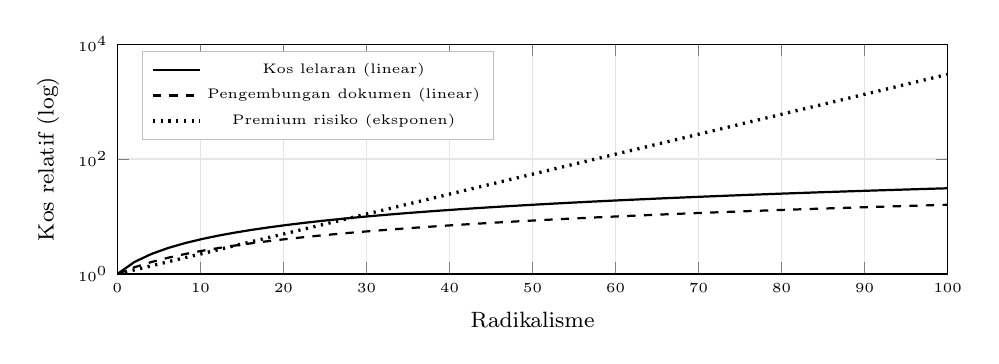
\begin{tikzpicture}
\begin{axis}[
    width=\columnwidth,
    height=4.5cm,
    xlabel={\footnotesize Radikalisme},
    ylabel={\footnotesize Kos relatif (log)},
    ymode=log,
    xmin=0, xmax=100,
    ymin=1, ymax=10000,
    grid=major,
    grid style={gray!20},
    legend style={at={(0.03,0.97)},anchor=north west,font=\tiny,draw=gray!50},
    tick label style={font=\tiny},
    label style={font=\footnotesize},
]
\addplot[black, thick, domain=0:100, samples=50] {1 + 0.3*x};
\addlegendentry{Kos lelaran (linear)}
\addplot[black, thick, dashed, domain=0:100, samples=50] {1 + 0.15*x};
\addlegendentry{Pengembungan dokumen (linear)}
\addplot[black, thick, dotted, line width=1.2pt, domain=0:100, samples=100] {exp(0.08*x)};
\addlegendentry{Premium risiko (eksponen)}
\end{axis}
\end{tikzpicture}
\caption{Peningkatan kos merentasi tiga saluran. Premium risiko mendominasi pada radikalisme tinggi.}
\label{fig:radicalism}
\end{figure}

Yang kritikal, ini bukan penapisan. Tiada dakwaan dilarang. Sistem meletakkan harga pada risiko (Jad.~\ref{tab:costs}).

\begin{table}[ht]
\centering
\caption{Perbandingan kos merentasi jenis dakwaan.}
\label{tab:costs}
\footnotesize
\begin{tabular}{@{}lcccc@{}}
\toprule
\textbf{Jenis} & \textbf{Lelaran} & \textbf{Dok} & \textbf{Yuran} & \textbf{Jumlah} \\
\midrule
Boleh dipercayai & $k_{\min}$ & $B_0$ & $P_{\min}$ & Rendah \\
Kontroversi & $k_{\text{med}}$ & $B_0{+}k\Delta$ & $\alpha e^{\beta d}$ & Sederhana \\
Radikal & $k_{\max}$ & $\gg B_0$ & $\gg P_{\min}$ & Sangat tinggi \\
Penipuan & $\to\infty$ & --- & --- & Tidak boleh diterbit \\
\bottomrule
\end{tabular}
\end{table}

% ============================================================
% 6. REPUTATION AND RISK
% ============================================================
\section{Penilaian Reputasi dan Risiko}

\subsection{Model Pengumpulan Reputasi}

Reputasi mempamerkan tiga sifat: \textbf{pengumpulan perlahan} (pertumbuhan beransur melalui tingkah laku konsisten), \textbf{pemusnahan pantas} (satu penipuan boleh mengurangkan skor secara malapetaka), dan \textbf{penilaian individu} (setiap pihak yang mengguna boleh menggunakan fungsi pengagregatan mereka sendiri).

\subsection{Autoriti Bereputasi}

Suatu Autoriti Bereputasi menyemak dakwaan dan, jika berpuas hati, menandatangani bersama---mempertaruhkan reputasinya sendiri (Raj.~\ref{fig:authority}). Ketaksimetrian ini adalah sengaja: memperoleh reputasi adalah perlahan (beransur $+\delta$ setiap sokongan jujur), sementara kehilangannya adalah malapetaka ($-\Delta \gg \delta$ setiap sokongan palsu; sebagai gambaran, contohnya, $+2\%$ berbanding $-70\%$). Strategi optimum sentiasa untuk menolak dakwaan yang mencurigakan. Nilai khusus $\delta$ dan $\Delta$ adalah parameter sistem.

\begin{figure}[ht]
\centering
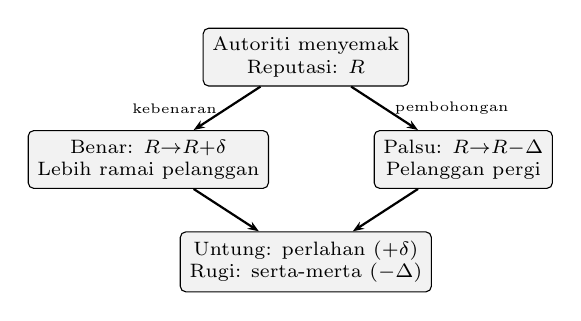
\begin{tikzpicture}[
    box/.style={draw, rounded corners=2pt, minimum width=2cm, minimum height=0.6cm, align=center, font=\scriptsize, fill=black!5},
    arr/.style={-{Stealth[length=4pt]}, thick}
]
\node[box] (exam) at (0,0) {Autoriti menyemak\\Reputasi: $R$};
\node[box] (true) at (-2,-1.3) {Benar: $R{\to}R{+}\delta$\\Lebih ramai pelanggan};
\node[box] (false) at (2,-1.3) {Palsu: $R{\to}R{-}\Delta$\\Pelanggan pergi};
\node[box] (insight) at (0,-2.6) {Untung: perlahan ($+\delta$)\\Rugi: serta-merta ($-\Delta$)};

\draw[arr] (exam) -- node[left,font=\tiny] {kebenaran} (true);
\draw[arr] (exam) -- node[right,font=\tiny] {pembohongan} (false);
\draw[arr] (true) -- (insight);
\draw[arr] (false) -- (insight);
\end{tikzpicture}
\caption{Autoriti Bereputasi---insentif tidak simetri.}
\label{fig:authority}
\end{figure}

\subsection{Reputasi Berbilang Dimensi}

Reputasi bukan skalar tetapi vektor merentasi berbilang dimensi: kebolehpercayaan kewangan, integriti peribadi, kecekapan profesional, penglibatan sivik, dan lain-lain (Raj.~\ref{fig:reputation-radar}). Penyedia penilaian yang berbeza memproyeksi vektor ini secara berbeza bergantung pada konteks---pemberi pinjaman mengutamakan kebolehpercayaan kewangan, majikan mengutamakan kecekapan profesional, jiran mengutamakan tingkah laku sivik. Tiada skor reputasi ``betul'' yang tunggal; hanya perspektif.

\begin{figure}[ht]
\centering
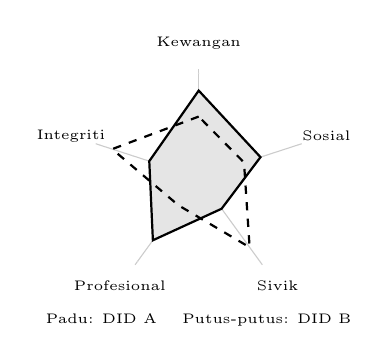
\begin{tikzpicture}[scale=0.55]
\foreach \a/\l in {90/Kewangan,162/Integriti,234/Profesional,306/Sivik,18/Sosial} {
  \draw[gray!40] (0,0) -- (\a:2.5);
  \node[font=\tiny, align=center] at (\a:3.1) {\l};
  \foreach \r in {0.8,1.6,2.4} {
    \fill[black!15] (\a:\r) circle (0.5pt);
  }
}
\draw[thick, fill=black!10] (90:2.0) -- (162:1.2) -- (234:1.8) -- (306:0.9) -- (18:1.5) -- cycle;
\draw[thick, dashed] (90:1.4) -- (162:2.1) -- (234:0.8) -- (306:2.0) -- (18:1.1) -- cycle;
\node[font=\tiny] at (0,-3.3) {Padu: DID A \quad Putus-putus: DID B};
\end{tikzpicture}
\caption{Vektor reputasi berbilang dimensi. DID berbeza mempamerkan profil berbeza merentasi dimensi.}
\label{fig:reputation-radar}
\end{figure}

\subsection{Penilaian Risiko Terdemokrasi}

RSN mendemokrasikan penilaian risiko bersistem---suatu keupayaan yang kini tertumpu dalam institusi kewangan tetapi terpakai jauh melangkaui perbankan. Konglomerat industri menaksir kebolehpercayaan pembekal, syarikat insurans meletakkan harga pada risiko tingkah laku, usaha wajar bagi penggabungan dan pengambilalihan, anggaran jangka hayat peralatan dalam pembuatan---di mana-mana risiko pihak lawan memerlukan penilaian, RSN menyediakan alternatif ternyahpusat yang dipacu pasaran. Suatu pasaran perkhidmatan tafsiran menterjemah data reputasi berbilang dimensi mentah kepada ringkasan yang boleh ditindaki, menjadikan penilaian pihak lawan boleh diakses oleh mana-mana peserta pada kos sut.

% ============================================================
% 7. CONSENSUS AND DISPUTE RESOLUTION
% ============================================================
\section{Konsensus dan Penyelesaian Pertikaian}

\subsection{Model Keadilan Ternyahpusat}

RSN merangka semula keadilan sebagai masalah rundingan dua hala. Ancaman kerosakan reputasi yang kekal dan boleh disahkan merupakan pencegah yang lebih berkesan daripada prosiding undang-undang yang tidak mampu ditanggung oleh pihak yang dimudaratkan.

\subsection{Konsensus Muncul}

Setiap peserta mengekalkan ambang kepuasan peribadi. Konsensus agregat rangkaian muncul sebagai purata statistik ribuan rundingan dua hala (Raj.~\ref{fig:consensus}). Suatu tindak balas jauh melebihi konsensus (kejam) adalah mahal untuk diterbitkan. Suatu tindak balas hampir dengan konsensus (berkadaran) adalah murah. Konsensus bukan suatu peraturan---ia adalah isyarat harga.

\begin{figure}[ht]
\centering
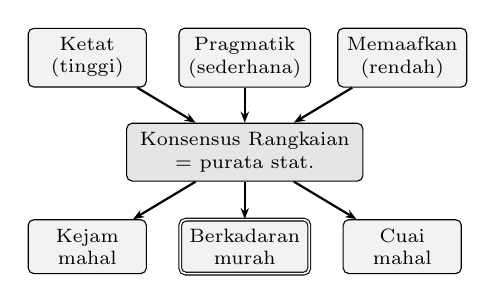
\begin{tikzpicture}[
    person/.style={draw, rounded corners=2pt, minimum width=1.5cm, minimum height=0.5cm, align=center, font=\scriptsize, fill=black!5},
    arr/.style={-{Stealth[length=4pt]}, thick}
]
\node[person] (a) at (-2,0) {Ketat\\(tinggi)};
\node[person] (b) at (0,0) {Pragmatik\\(sederhana)};
\node[person] (c) at (2,0) {Memaafkan\\(rendah)};
\node[person, fill=black!10, minimum width=3cm] (cons) at (0,-1.2) {Konsensus Rangkaian\\= purata stat.};
\node[person] (exp) at (-2,-2.4) {Kejam\\mahal};
\node[person, double] (prop) at (0,-2.4) {Berkadaran\\murah};
\node[person] (neg) at (2,-2.4) {Cuai\\mahal};

\draw[arr] (a) -- (cons);
\draw[arr] (b) -- (cons);
\draw[arr] (c) -- (cons);
\draw[arr] (cons) -- (exp);
\draw[arr] (cons) -- (prop);
\draw[arr] (cons) -- (neg);
\end{tikzpicture}
\caption{Konsensus muncul daripada ambang kepuasan individu.}
\label{fig:consensus}
\end{figure}

\subsection{Penentukuran Hukuman}

Setiap Pemegang DID mengisytiharkan tindak balas secara terbuka terhadap kategori salah laku tertentu. Pengisytiharan yang terlalu keras atau terlalu lembut menarik isyarat reputasi negatif. Pengisytiharan yang berkadaran diterima tanpa geseran---suatu sistem hukuman yang menentukur diri sendiri.

Pengisytiharan konsensus itu sendiri tertakluk kepada pengesanan kemunafikan: berkomit secara pengisytiharan kepada suatu kedudukan konsensus sambil bertingkah laku secara tidak konsisten merupakan kesalahan reputasi yang lebih teruk daripada sisihan asas, kerana ia menunjukkan penipuan yang disengajakan.

\subsection{Pewakilan}

Semua aktiviti dalam suatu DID---dengan satu pengecualian---boleh diwakilkan kepada DID lain. \textbf{Peranan Subjek---DID yang tingkah lakunya menjadi subjek dakwaan---tidak boleh diwakilkan; ia terikat secara tidak boleh dipindah kepada pemegang identiti yang dirujuk oleh dakwaan.} Peranan aktif yang lain---Pengeluar, Autoriti, Saksi, Pengesah---boleh dipindahkan kepada DID wakil yang ditetapkan, sama ada untuk pengesahan, penyerahan dakwaan, penyertaan konsensus, atau penyelesaian pertikaian. Pewakilan boleh dibatalkan pada bila-bila masa. Ini membolehkan pengkhususan (contohnya, perkhidmatan pengesahan profesional) sementara Pemegang mengekalkan kawalan dan tanggungjawab muktamad. Pewakilan terpakai merentasi seluruh sistem dan penting untuk keterukuran.

\subsection{Daripada Moraliti Individu kepada Kontrak Sosial yang Muncul}

Dasar diisytihar setiap DID mewakili pemformalan moraliti individu: apa yang dianggap boleh diterima oleh Pemegang, bagaimana mereka bertindak balas terhadap tingkah laku tertentu, apa yang mereka kehendaki daripada pihak lawan. Dasar-dasar ini tidak dikenakan oleh pereka sistem---ia dipilih oleh setiap peserta dan diungkapkan dalam bentuk boleh dibaca mesin.

Pemformalan ini membolehkan kemunculan tiga peringkat. Pertama, moraliti individu dikodkan sebagai \textbf{dasar}---satu set peraturan diisytihar, ambang, dan fungsi tindak balas yang DID komit untuk ikuti. Kedua, agregat semua dasar merentasi rangkaian menghasilkan \textbf{etika muncul}---norma yang boleh diperhati secara statistik yang tiada seorang peserta pun mereka tetapi yang timbul daripada interaksi ribuan kedudukan moral individu~\cite{durkheim1893}. Ketiga, etika muncul ini, diungkapkan sebagai norma tingkah laku dikongsi yang dikuatkuasakan melalui isyarat harga dua hala, membentuk \textbf{kontrak sosial yang boleh diukur}---bukan suatu binaan teori yang tiada sesiapa tandatangani~\cite{rawls1971}, tetapi satu set peraturan yang boleh diperhati secara empirik dan disokong oleh tingkah laku sebenar.

Proses ini mencerminkan penemuan daripada teori asas moral~\cite{haidt2012}: moraliti manusia adalah intuitif, pluralistik, dan berbeza-beza mengikut budaya. RSN tidak memerlukan konsensus moral sebagai input; ia menghasilkan konsensus tingkah laku sebagai output. Kontrak sosial yang terhasil tidak statik---ia berkembang apabila peserta menyertai, keluar, dan menyesuaikan dasar mereka sebagai tindak balas kepada maklum balas rangkaian. Tidak seperti teori kontrak sosial klasik, kontrak ini boleh dibatalkan, boleh diperhati, dan boleh dikuatkuasakan tanpa penguasa berdaulat.

% ============================================================
% 8. ECONOMIC MODEL
% ============================================================
\section{Model Ekonomi}

Seksyen sebelumnya menerangkan suatu alat---mekanisme pengesahan RSN, struktur kos, dan konsensus muncul. Seksyen ini menerangkan suatu metodologi untuk menggunakan alat ini pada peralihan fiskal dan tadbir urus. Alat ini adalah tujuan umum; metodologi di bawah ialah satu aplikasi yang mungkin.

\subsection{Struktur Insentif}

Reputasi sebagai modal mewujudkan insentif langsung untuk tingkah laku jujur. Dalam operasi biasa, peserta membina reputasi secara semula jadi melalui transaksi harian dan komitmen yang dipenuhi. Perbelanjaan utama adalah pada dakwaan \emph{negatif}---merekodkan kemudaratan yang dilakukan oleh orang lain. Ketaksimetrian ini memberi insentif kepada tingkah laku yang berguna dan boleh dipercayai: bersikap jujur tidak memakan kos tambahan, sementara bersikap memudaratkan mewujudkan jejak berdokumen yang orang lain akan bayar untuk mengekalkannya. Kemunafikan---mengisytiharkan peraturan tanpa mengikutinya---ialah mod kegagalan yang paling mahal, kerana ia menunjukkan penipuan yang disengajakan.

\subsection{Sistem Fiskal Selari}

Tiga komponen membolehkan tekanan persaingan: (1)~\textbf{Cukai Ringkas}---suatu kadar berkadaran tunggal tanpa pengecualian, pada mulanya sedikit di bawah kadar berkesan sedia ada; (2)~\textbf{Pendaftaran Perbelanjaan Elektronik (ESR)}---membalikkan model EET Czech supaya rakyat memantau perbelanjaan negara; (3)~\textbf{Peruntukan Cukai Diarahkan Rakyat}---bermula pada beberapa peratus dalam tahun pertama dan mencapai, selepas sedekad, di mana-mana antara angka dua digit rendah hingga migrasi penuh kepada sistem diarahkan rakyat, bergantung pada kadar penerimaan. Tempo sebenar bergantung pada kelajuan kemunculan alternatif pasaran bebas kepada perkhidmatan negara dan pada kesanggupan negara untuk bekerjasama dengan peralihan; fungsi masa tidak semestinya linear, dan tiada sebab untuk menetapkan had atas di mana penerimaan mungkin akhirnya tiba.

% ============================================================
% 9. MIGRATION PATH
% ============================================================
\section{Laluan Peralihan}

Peralihan diteruskan melalui tiga fasa (Raj.~\ref{fig:migration}): \textbf{Fasa~1: Lapisan Tindanan} (RSN sebagai lapisan maklumat, negara sebagai penyedia tunggal), \textbf{Fasa~2: Persaingan} (RSN menyediakan alternatif berfungsi, penggunaan dwi-sistem), dan \textbf{Fasa~3: Peralihan} (RSN mengatasi kesetaraan negara, migrasi sukarela). Peralihan boleh diterbalikkan pada setiap peringkat.

\begin{figure}[ht]
\centering
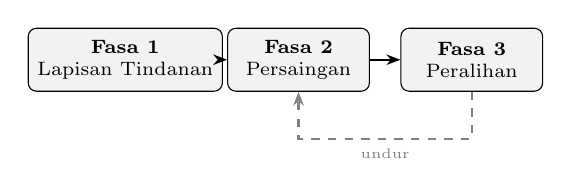
\begin{tikzpicture}[
    phase/.style={draw, rounded corners=3pt, minimum width=1.8cm, minimum height=0.8cm, align=center, font=\scriptsize, fill=black!5},
    arr/.style={-{Stealth[length=5pt]}, thick}
]
\node[phase] (p1) at (0,0) {\textbf{Fasa 1}\\Lapisan Tindanan};
\node[phase] (p2) at (2.2,0) {\textbf{Fasa 2}\\Persaingan};
\node[phase] (p3) at (4.4,0) {\textbf{Fasa 3}\\Peralihan};

\draw[arr] (p1) -- (p2);
\draw[arr] (p2) -- (p3);
\draw[arr, dashed, gray] (p3.south) -- ++(0,-0.6) -| node[below,font=\tiny,pos=0.25] {undur} (p2.south);
\end{tikzpicture}
\caption{Peralihan tiga fasa---boleh diterbalikkan pada setiap peringkat.}
\label{fig:migration}
\end{figure}

Mekanisme tekanan utama adalah fiskal: apabila pembayar cukai bersyarat mencapai suatu ``minoriti signifikan ekonomi $X$''---suatu kumpulan yang cukup besar sehingga penindasan terhadapnya menyebabkan kerosakan ekonomi yang tidak remeh dan ketidakpatuhan awam menjadi ancaman yang boleh dipercayai---negara memasuki rundingan. Sebagai gambaran, kami menggunakan $X \approx 15\%$ daripada KDNK, tetapi ambang sebenar bergantung pada ekonomi tertentu.

% ============================================================
% 10. SECURITY ANALYSIS
% ============================================================
\section{Analisis Keselamatan}

Kami mempertimbangkan lima kategori musuh: pelaku jahat individu, kumpulan tersusun, musuh korporat, musuh peringkat negara, dan musuh peringkat protokol.

\textbf{Ketahanan Sybil}~\cite{douceur2002}. Membina reputasi memerlukan interaksi yang berterusan dan boleh disahkan. Kos serangan Sybil yang berjaya berskala secara linear dengan identiti palsu dan secara kuadratik dengan tahap reputasi sasaran. Mengendalikan berbilang DID secara selari adalah mungkin tetapi mahal secara reka bentuk---setiap identiti mesti mengumpul reputasi secara bebas melalui aktiviti tulen. Dalam masyarakat bebas, kos ini menghalang penyalahgunaan sambil lewa; dalam kediktatoran, DID selari menjadi alat kelangsungan hidup yang membolehkan penentangan berpetak, penyelarasan bawah tanah, dan pelayaran pasaran gelap yang lebih selamat.

\textbf{Pertahanan pakatan sulit.} Corak sokongan bersama dalam kalangan kumpulan tertutup boleh dikesan melalui analisis graf sosial. Fungsi pengagregatan reputasi mendiskaun dakwaan daripada sumber yang berkelompok rapat.

\textbf{Musuh peringkat negara.} Penghalaan onion, ketiadaan infrastruktur terpusat, dan pengagihan peranan Pengesah merentasi asas peserta memastikan bahawa penindasan memerlukan langkah yang tidak berkadaran dengan sebarang manfaat.

\textbf{Privasi berbanding kebertanggungjawaban.} Kesamaran---jalan tengah antara kerahsiaan dan pendedahan identiti---membolehkan DID mengumpul reputasi yang bermakna tanpa mendedahkan identiti dunia nyata Pemegang.

% ============================================================
% 11. PRIVACY
% ============================================================
\section{Pertimbangan Privasi}

Model privasi RSN dibina di atas kesamaran. Pemegang mengawal pendedahan identiti: minimum (samaran tulen), terpilih (kelayakan tertentu dipautkan), atau penuh (identiti undang-undang dikaitkan). Dakwaan yang diterbitkan adalah kekal---sistem menyokong pembetulan kontekstual tetapi bukan pemadaman. Seorang Pemegang boleh meninggalkan DID yang terkompromi dan bermula semula, melepaskan reputasi yang terkumpul.

% ============================================================
% 12. RELATED WORK
% ============================================================
\section{Kerja Berkaitan}

Spesifikasi W3C DID Core~\cite{did2022} dan Rangkaian Ceramic~\cite{ceramic2023} menyediakan asas identiti. EigenTrust~\cite{kamvar2003} menunjukkan pengagregatan reputasi teragih tanpa autoriti pusat. SBT~\cite{weyl2022} memperkenalkan token sosial tidak boleh dipindah milik. RSN berbeza dalam penekanannya pada kos ekonomi sebagai penapis kualiti dan mekanismenya untuk meletakkan harga pada radikalisme.

DAO~\cite{buterin2014} dan pengundian kuadratik~\cite{buterin2019} menunjukkan kebolehlaksanaan tadbir urus ternyahpusat. RSN memperoleh konsensus daripada rundingan harga dua hala dan bukannya pengundian.

Cadangan ini bertumpu pada teori anarko-kapitalis~\cite{rothbard1973,hoppe2001} untuk penyediaan perkhidmatan persendirian tetapi menyimpang dalam dua aspek kritikal: ia mereka bentuk untuk dendam dan dorongan pembalasan dan bukannya mengandaikan kerasionalan, dan ia mencadangkan peralihan beransur-ansur dan bukannya revolusi. Konsep kontrak sosial muncul mempunyai pendahulunya dalam teori susunan spontan Hayek~\cite{hayek1973}.

\textbf{Anarko-agorisme.} RSN berkongsi persamaan yang ketara dengan kontra-ekonomi agoris~\cite{konkin2006}---terutamanya penekanan pada membina institusi selari dan pertukaran sukarela. Walau bagaimanapun, agorisme cenderung mengandaikan kepentingan diri rasional sebagai mekanisme penyelarasan yang mencukupi dan sering kekurangan laluan peralihan yang konkrit daripada struktur negara sedia ada. RSN secara eksplisit menggabungkan kecenderungan tingkah laku tidak rasional dan menyediakan mekanisme tekanan fiskal untuk peralihan beransur-ansur.

\textbf{Meritokrasi.} RSN mungkin mewakili penerangan berfungsi pertama tentang bagaimana meritokrasi~\cite{young1958} boleh muncul sebagai sifat sistemik dan bukannya slogan. Sistem meritokratik tradisional gagal kerana ia memerlukan autoriti pusat untuk mentakrif dan menguatkuasakan ``merit.'' Dalam RSN, merit muncul daripada penilaian dua hala: mereka yang menyampaikan nilai mengumpul reputasi; tiada jawatankuasa memutuskan siapa yang mempunyai merit.

\textbf{Harta sebagai keistimewaan.} RSN menyimpang secara asas daripada layanan anarko-kapitalis dan mazhab Austria terhadap hak harta sebagai semula jadi dan mutlak. Dalam kerangka RSN, harta ialah suatu \emph{keistimewaan}---suatu pengiktirafan sosial yang boleh, dalam kes melampau, ditarik balik oleh komuniti apabila seorang peserta melanggar norma dikongsi secara asas (pengkhianatan, keengganan mempertahankan komuniti dalam krisis kewujudan, eksploitasi bersistem). Ini bukan perampasan negara tetapi penarikan balik pengiktirafan sosial oleh rangkaian hubungan dua hala.

% ============================================================
% 13. LIMITATIONS
% ============================================================
\section{Perbincangan dan Batasan}

\textbf{Permulaan sejuk.} Nilai RSN bergantung pada kesan rangkaian; pengguna awal menghadapi nilai terhad sehingga penyertaan mencapai suatu ambang. Walau bagaimanapun, walaupun dari peringkat awal, rangkaian DID berfungsi sebagai sumber maklumat tambahan yang berguna. Penilaian reputasi awal dan penaksiran autoriti dijangka berkembang secara beransur-ansur dengan kecanggihan yang meningkat.

\textbf{Anti-lintah dan kawalan akses.} DID sasaran boleh mengenakan yuran berperingkat dan sekatan akses ke atas pertanyaan daripada DID reputasi rendah. Ini bukan binari tetapi skala berterusan: semakin sedikit reputasi yang dimiliki oleh suatu DID yang bertanya, semakin sedikit maklumat yang diterima, semakin lama ia menunggu, dan semakin banyak ia membayar. Mekanisme ini memberi insentif kepada penyertaan tulen berbanding penggunaan pasif.

\textbf{Ketidaksamaan akses.} Kos menerbitkan dakwaan mungkin menapis keluar rungutan yang sah daripada peserta yang kurang bernasib baik dari segi ekonomi. Mitigasi: setiap peserta serentak berkhidmat sebagai pengesah berpotensi (atau mewakilkan peranan ini) dan memperoleh yuran pengesahan. Dalam ufuk masa yang mencukupi, seorang peserta bukan radikal sepatutnya menghampiri kenetralan kewangan---pendapatan pengesahan lebih kurang mengimbangi kos penerbitan. Ini adalah jangkaan statistik, bukan jaminan.

\textbf{Ketidaksamaan reputasi.} Pengguna awal mengumpul kelebihan yang mungkin mewujudkan halangan bagi pendatang lewat. Walau bagaimanapun, penilaian reputasi dilakukan oleh penyedia pihak ketiga yang mungkin memilih untuk mengurangkan kelebihan penggerak pertama melalui algoritma pengagregatan mereka. Menjadi yang pertama dengan reputasi baik ialah suatu kelebihan ekonomi perbandingan yang sah---dan itu adalah secara reka bentuk.

\textbf{Persoalan terbuka.} Fungsi kos optimum, piawaian pengagregatan, tadbir urus protokol, dan interaksi dengan data reputasi sintetik yang dijana AI kekal sebagai bidang untuk kerja masa depan.

Kertas ini tidak mendakwa bahawa RSN akan menghasilkan hasil optimum dalam semua keadaan. Ia mendakwa bahawa RSN mewakili suatu alternatif yang \emph{boleh dilaksanakan}---boleh dilaksanakan secara teknikal, mampan sendiri dari segi ekonomi, dan serasi secara sosial dengan kecenderungan tingkah laku manusia sebagaimana ia sebenarnya wujud.

% ============================================================
% 14. CONCLUSION
% ============================================================
\section{Kesimpulan}

Kertas ini telah membentangkan Rangkaian Sosial Reputasi, suatu protokol ternyahpusat yang membolehkan pertukaran reputasi samaran yang boleh disahkan. Prinsip Radikalisme Mahal memastikan bahawa dakwaan penipuan diberi harga terkeluar tanpa penapisan. Laluan peralihan yang dicadangkan membolehkan peralihan beransur-ansur dan boleh diterbalikkan daripada institusi sedia ada. Reka bentuk ini menggabungkan sifat semula jadi manusia sebagaimana adanya---termasuk kepicikan, dendam, dan keinginan untuk kepuasan pembalasan---dan bukannya memerlukan transformasi ideologi. Hasilnya bukan utopia tetapi suatu sistem di mana keadilan boleh diakses, reputasi diperoleh, dan kos salah laku ditanggung oleh pihak yang menyebabkannya.

% ============================================================
% REFERENCES
% ============================================================
\bibliography{references}

\end{document}
